\begin{problem}[19]
计论方形空心简支梁的挠度分布, 若用实心梁来模拟, 要求符合什么条件?
\end{problem}
% --------------------------------------------------------------------
\begin{solution}
\begin{minipage}[c]{0.7\linewidth}
由\hyperref[problem:17]{17}题式(\ref{eq:17-wl})结论, 可知若用实心梁来模拟方形空心简支梁的挠度分布, 不必要求模型的截面形状遵守几何相似的条件, 只要求截面矩满足
\end{minipage}
\begin{minipage}[c]{0.3\linewidth}
\begin{center}
\usetikzlibrary{calc,intersections,through,backgrounds}
\usetikzlibrary{decorations.pathreplacing,decorations.pathmorphing,arrows}
\usetikzlibrary{shapes}
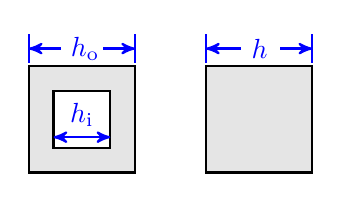
\begin{tikzpicture}[scale=0.9]
\draw[thick,fill=gray!20] (-0.75,-0.75) rectangle(0.75,0.75);
\draw[thick,fill=white]  (-0.4,-0.4) rectangle (0.4,0.4);


\draw[thick,blue,<-,>=stealth'] (-0.75,0.8)--(-0.75,1.2) (0.75,0.8)--(0.75,1.2) (-0.75,1)--(-0.3,1) node[right]{$h_\mathrm{o}$};
\draw[thick,blue,->,>=stealth'] (0.3,1)--(0.75,1) ;
\draw[thick,blue,<->,>=stealth'] (-0.4,-0.25)--(0.4,-0.25) node[midway,above]{$h_\mathrm{i}$} ;


\draw[thick,fill=gray!20] (1.75,-0.75) rectangle(3.25,0.75);
\draw[thick,blue,<-,>=stealth'] (1.75,0.8)--(1.75,1.2) (3.25,0.8)--(3.25,1.2) (1.75,1)--(2.25,1) node[right]{$h$};
\draw[thick,blue,->,>=stealth'] (2.8,1)--(3.25,1) ;
\end{tikzpicture}
\end{center}
\end{minipage}
\[
\bigg(\frac{q_ml^3}{EI}\bigg)_\mathrm{m} = \bigg(\frac{q_ml^3}{EI}\bigg)_\mathrm{p}
\]
对于方形实心简支梁和方形空心简支梁, 截面矩分别为:
\begin{itemize}
\item \textbf{方形实心简支梁}: 边长为$h$, 则$I_\mathrm{m} = h^4/12$.
\item \textbf{方形空心简支梁}: 内外边长分别为$h_\mathrm{i}$, $h_\mathrm{o}$, 则$I_\mathrm{p}=(h_\mathrm{o}^4-h_\mathrm{i}^4)/12$.
\end{itemize}
因此若用实心梁来模拟方形空心简支梁的挠度分布需满足
\[
\Bigg[\frac{q_ml^3}{Eh^4}\Bigg]_\mathrm{m} = \Bigg[\frac{q_ml^3}{E\big(h_\mathrm{o}^4-h_\mathrm{i}^4\big)}\Bigg]_\mathrm{p}
\]
\end{solution}
\label{problem:19}
